\section{Responsive Search}\label{RSearch}
\begin{center}
    \userstory{As a User I would like the Pictosearch application to feel more responsive when I search for pictograms, such that I don't feel like nothing happens.}
\end{center}

The task was created because the customers expressed concern for the reactiveness of the Pictosearch application --- it sometimes felt slow and customers said it felt like nothing was happening.
The Pictosearch application is used whenever the user needs to find a certain pictogram for other applications such as the Week Schedule or the Sequence application.
It is a problem that the users feel like the application is slow and that it does not react quickly to what the user is doing, especially in an application used often by other applications of GIRAF.
It is important that responses from a mobile application are given within a few seconds, as mentioned in~\cite{Roto:2005:NNF:1062745.1062747}, if an application spends more than four seconds to load or respond then other feedback than visual should be used.
Therefore the amount of time spent waiting for the application should be reduced, such that there is no need for using other methods of feedback when the search finally returns.
According to Constantine and Lockwood in their book \enquote{Software for Use: A Practical Guide to the Models and Methods of Usage-Centered Design} \cite{DESIGNBOOK}, a design principle regarding feedback is as follows:

\begin{displayquote}
\textit{Keep users informed of actions or interpretations, changes of state or condition and errors or exceptions that are relevant and of interest to the user through clear, concise, and unambiguous language familiar to users\cite[p.~57]{DESIGNBOOK}.}
\end{displayquote}

Therefore it is decided that the Pictosearch application should give visual feedback whenever an action occurs.
The application should respond to the users action more often than what it does now to increase how responsive the application feels to the user.

The current version of the Pictosearch application searches whenever the user taps the search button on either the on-screen keyboard or in the GUI of the application.
The search button is located in the middle of the screen, to the left of the search field as can be seen on \myref{fig:screenshot_startup}.

\begin{figure}[ht]
    \centering
    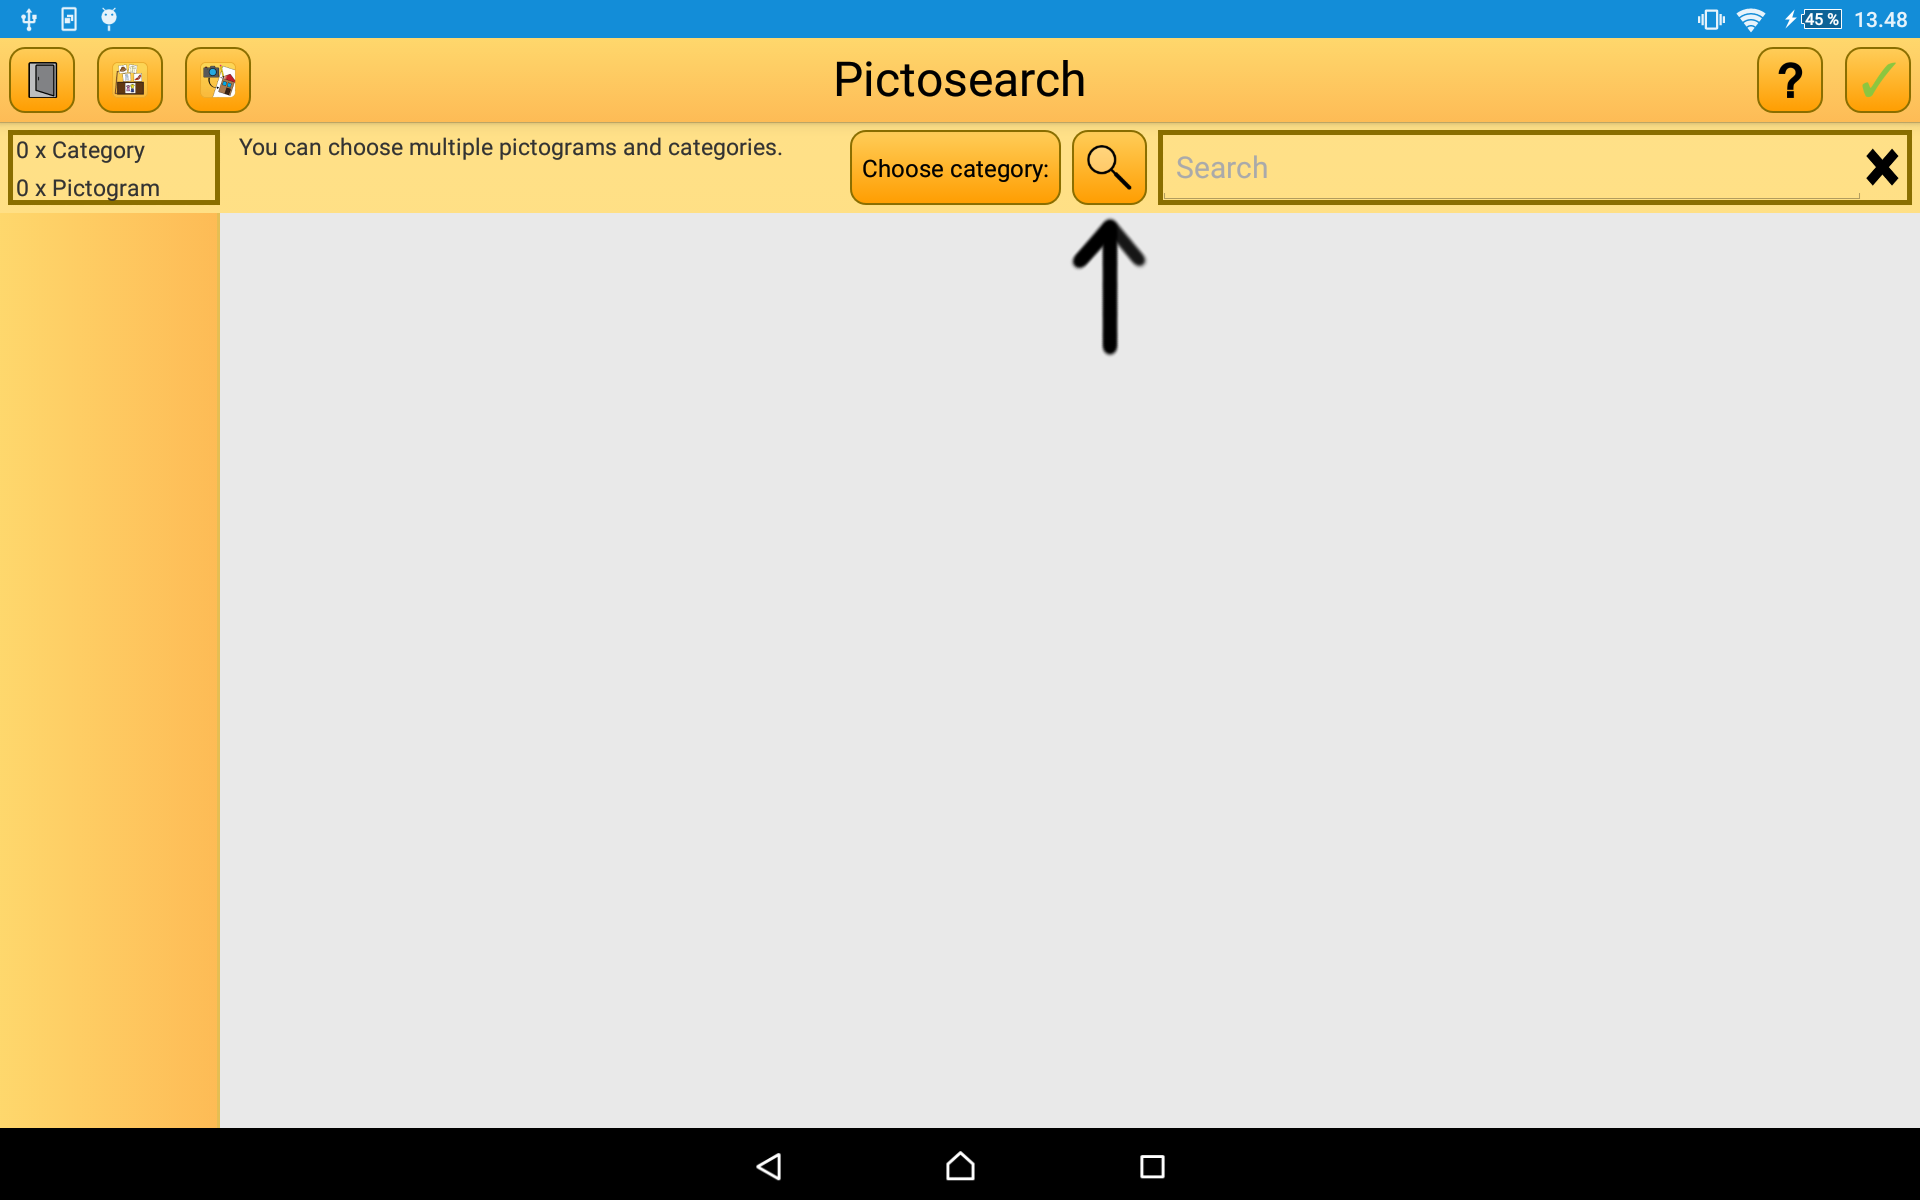
\includegraphics[width=0.8\textwidth]{figures/img/screenshots/old_startup.png}
    \caption{Screenshot of the initial view presented to the user when launching Pictosearch, with the search button highlighted.}\label{fig:screenshot_startup}
\end{figure}
\noindent
The screenshot also shows the view of the application as it is opened, completely empty with no information.

\begin{figure}[ht]
    \centering
    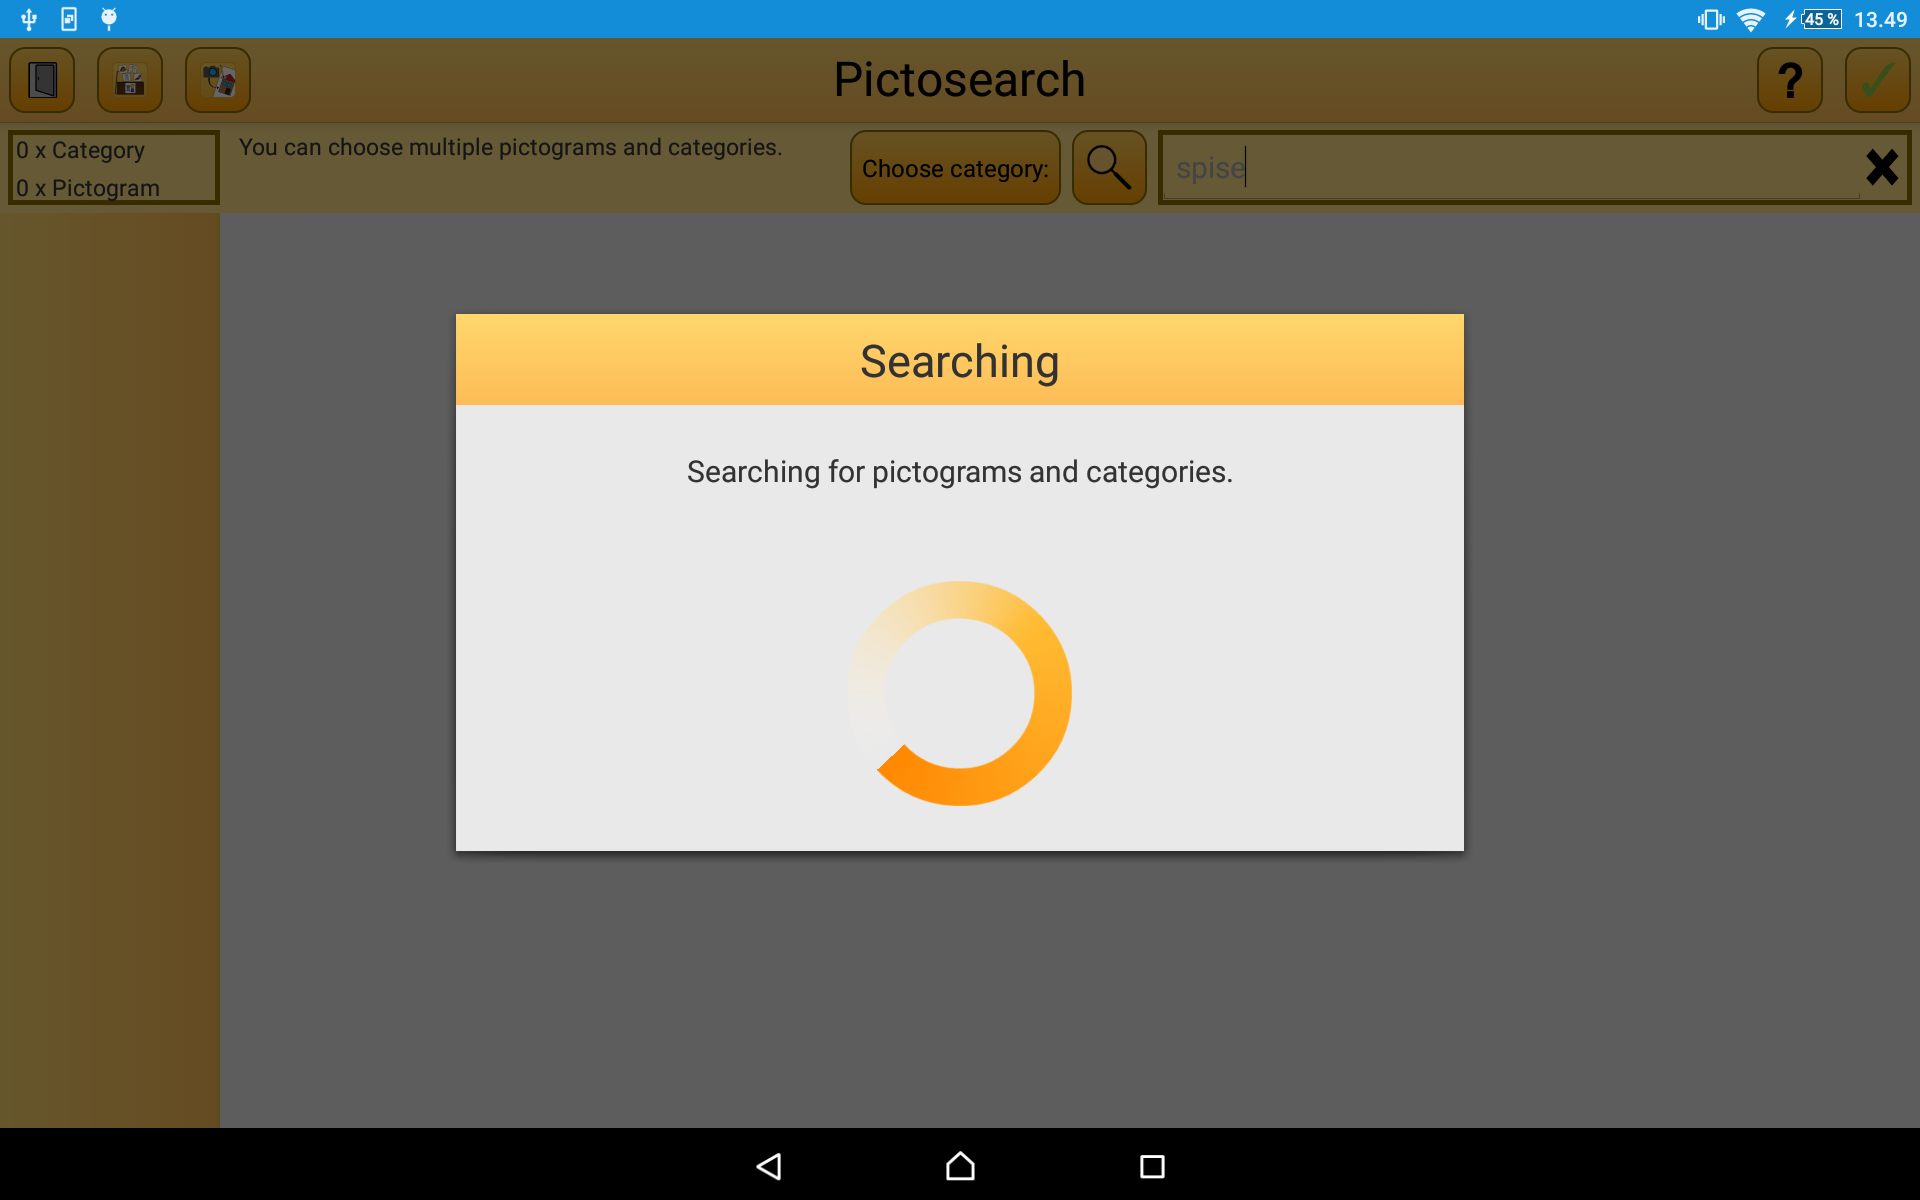
\includegraphics[width=0.8\textwidth]{figures/img/screenshots/old_dialog.png}
    \caption{Screenshot of the search spinner shown while searching in Pictosearch.}\label{fig:screenshot_searchspinner}
\end{figure}

In the new version, a search is made whenever the text in the searchfield is changed.
Instead of the big slow search spinner, which blackened out and locked the screen, shown on \myref{fig:screenshot_searchspinner}, a new smaller text message is instead displayed which tells the user that the application is searching and what it is searching for.
The current version would also remove the on--screen keyboard when it would search, this only happens in the new version whenever the search button is pressed or the user taps somewhere else, i.e. not on the keyboard.
The application can take input while searching because it is implemented as an async task, i.e. in its own thread.
Because of this any new search is queued behind the current search query, and as such the results of the latest search will be waiting for the results of the previous searches.
This is fixed by a simple change of calling \texttt{AsyncTask.cancel()}, which is a thread.cancellation method, that stops the execution of the ongoing thread and makes it possible to start a new call immediately, with the updated search string, and therefore eliminating the queue.
Because of this anytime a keystroke is made on the keyboard something will happen on the display other than simply filling out the search--field.
When the user types a letter in the textfield, the application will search for the text currently in the text field and display the text as seen on \myref{fig:screenshot_newsearch} explaining what is being searched for.
This fulfills the principle of giving feedback to the user when an action occurs, such that the user knows what is happening behind the scenes.
When the search returns the pictograms will be shown instead of the text message, with the keyboard still visible.

\begin{figure}[ht]
    \centering
    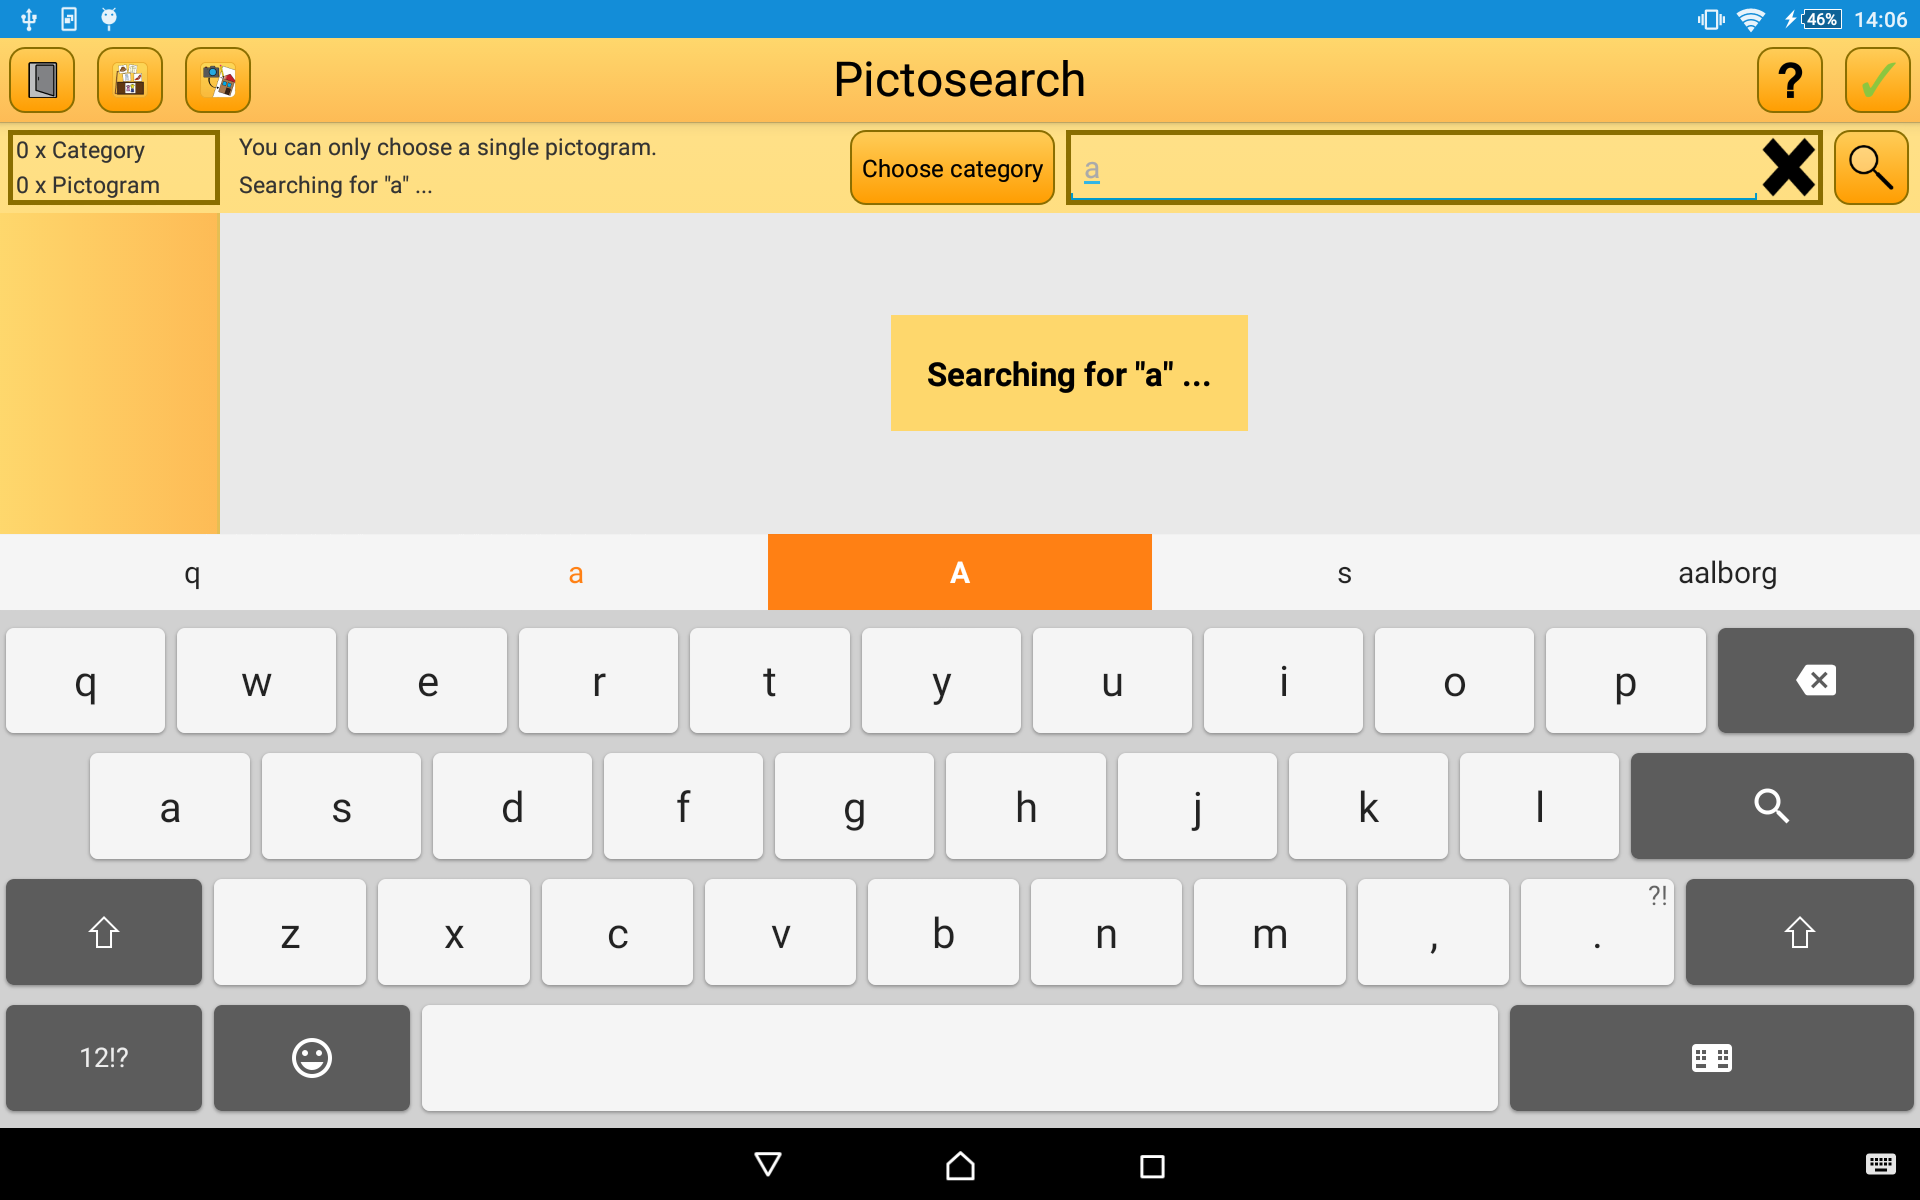
\includegraphics[width=0.8\textwidth]{figures/img/screenshots/new_dialog.png}
    \caption{Screenshot of the new search information, while searching.}\label{fig:screenshot_newsearch}
\end{figure}

This means that there is near instantaneous feedback for the user, which might give the feeling that the application is reacting to whatever the user is doing, and it might no longer feel to users like nothing is happening.
Previously the user would be waiting forever if he thought a search would be performed, when text was entered into the search--field, such as Google does.
The new approach hereby provides search feedback significantly closer to the aforementioned 4 second limit.
Actually, the query which results in the largest amount of pictograms is a search for the character \enquote{s}, it returns 1932 pictograms and takes approximately 4 seconds on the relatively slow Lenovo tablet provided by the University --- as this is the worst case regarding search time, the average use case will always be faster than 4 seconds.

The search button can still be used, and will bring up the old search spinner as usually, this is done so that \enquote{refreshing} a search result will provide feedback.
Moreover the button has been moved from the middle of the display to the right side of the display as can be seen on \myref{fig:screenshot_newstartup}.
This is a better fit as it resembles other common search engines such as Google Search, and it is also the recommended way to display a search--field according to the Niels Norman Group\footnote{\url{https://www.nngroup.com/articles/magnifying-glass-icon/}}.
Furthermore according to the principles of Constantine and Lockwood, structuring the interface is important such that it is for example recognisable:

\begin{displayquote}
\textit{Organize the user interface purposefully, in meaningful and useful ways based on clear, consistent models that are apparent and recognizable to users, putting related things together and separating unrelated things, differentiating dissimilar things and making similar things resemble one
another.}\cite[p.~51]{DESIGNBOOK}
\end{displayquote}
\noindent
Therefore using a familiar position of the button is a better fit than placing it in the middle of the screen as in the current version.

Another thing we noticed was that the clear search field button was visible all the time even though no text was in the search--field.
This has been removed and it is now only visible when there is text in the search--field i.e. when the actoion is available, as can be seen on \myref{fig:screenshot_newstartup} and it is still there on \myref{fig:screenshot_newsearch}.
This has been done because of another design pricinple by Constantine and Lockwood:

\begin{displayquote}
\textit{Keep all needed options and materials for a given task visible without distracting the user with extraneous or redundant information.} \cite[p.~55]{DESIGNBOOK}
\end{displayquote}

\begin{figure}[ht]
    \centering
    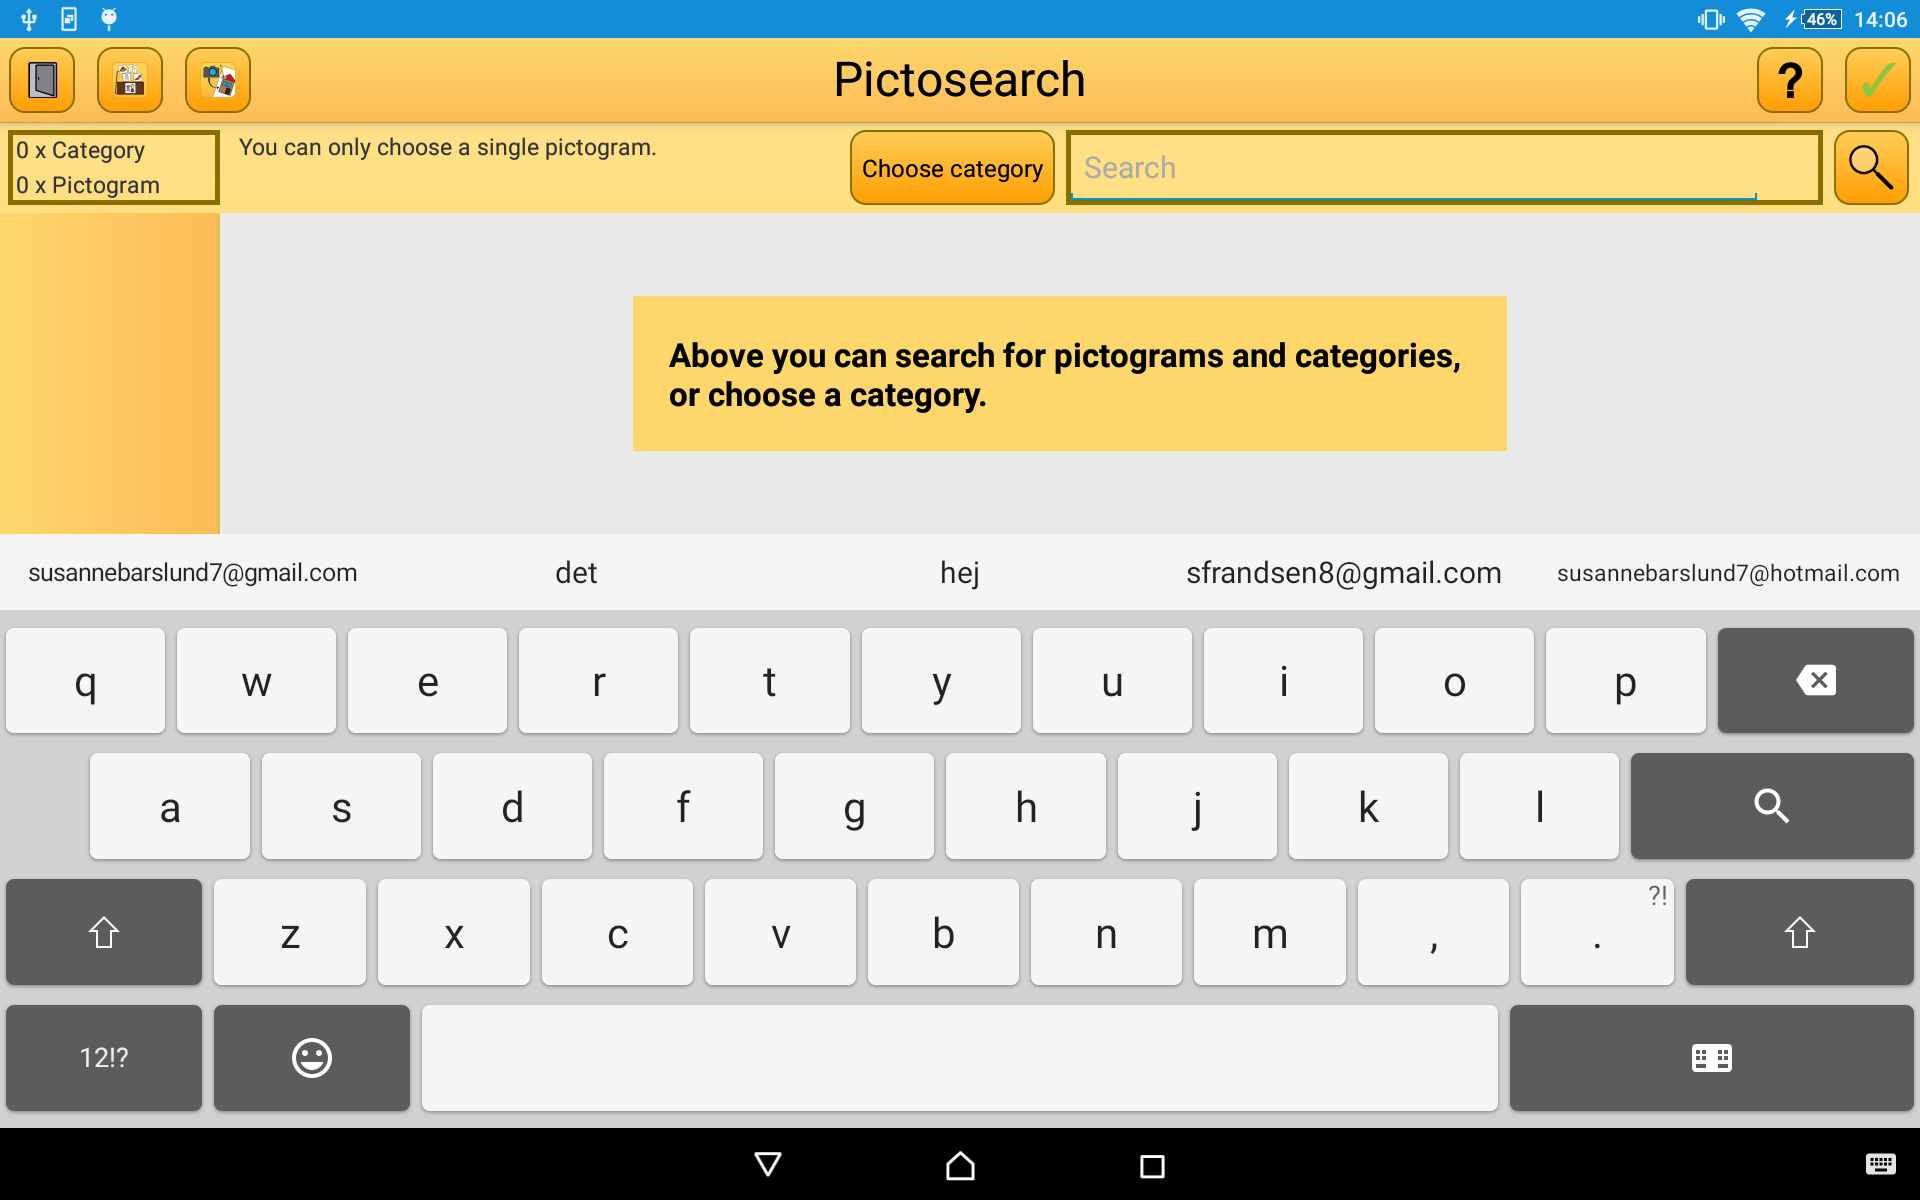
\includegraphics[width=0.8\textwidth]{figures/img/screenshots/new_startup.png}
    \caption{Screenshot of the new initial view in Pictosearch.}\label{fig:screenshot_newstartup}
\end{figure}

